%%%%%%%%%%%%%%%%%%%%%%%%%%%%%%%%%%%%%%%%%%%%%%%%%%%%%%%%%%%

%% document class
\documentclass[12pt,a4paper]{article}

%% packages
%% packages

\usepackage{blindtext} % needed for creating dummy text passages
\usepackage{amsmath} % needed for command eqref
\usepackage{amssymb} % needed for math fonts
\usepackage{amsthm} % To format theorems, lemmas, proofs, etc
\usepackage{mathtools}  % To annotate equation terms using \mathclap

\usepackage{pifont}% For ticks and crosses as defined in the newcommands below. More info at http://ctan.org/pkg/pifont
\newcommand{\cmark}{\ding{51}}%
\newcommand{\xmark}{\ding{55}}%

%%%%%%%%%%%%%%%%%%%%%%%%%%%%%%%%%%%%%%%%%%%%%%%%%%%%%%%%%%%
\usepackage[
	colorlinks=true
	,breaklinks %in case some labels are too long and may span several pages, e.g. in List of Figures, etc.
	]{hyperref} % needed for creating hyperlinks in the document, the option colorlinks=true gets rid of the awful boxes, breaklinks breaks long links (list of figures), and ngerman sets everything for german as default hyperlinks language
\usepackage[hyphenbreaks]{breakurl} % ben�tigt f�r das Brechen von URLs in Literaturreferenzen, hyphenbreaks auch bei links, die �ber eine Seite gehen (mit hyphenation).

\usepackage{xcolor}
\definecolor{c1}{rgb}{0,0,1} % blue
\definecolor{c2}{rgb}{0,0.3,0.9} % light blue
\definecolor{c3}{rgb}{0.3,0,0.9} % red blue
\hypersetup{
    linkcolor={c1}, % internal links
    citecolor={c2}, % citations
    urlcolor={c3} % external links/urls
}

%\usepackage{cite} % needed for cite
\usepackage[round,authoryear]{natbib} % needed for cite and abbrvnat bibliography style
\usepackage[nottoc]{tocbibind} % needed for displaying table of contents, bibliography, index and other in the table of contents. 'nottoc' is to exclude the phreases "table of contents" from the table of contents.
%%%%%%%%%%%%%%%%%%%%%%%%%%%%%%%%%%%%%%%%%%%%%%%%%%%%%%%%%%%

\usepackage{graphicx} % needed for \includegraphics
\usepackage{subcaption} % for creating subfigures (side-by-side) and captioning them
\usepackage{float}	% to insert tables at precise position of code with [H] specifier.
\usepackage{longtable} % needed for long tables over pages
\usepackage{bigstrut} % needed for the command \bigstrut
\usepackage{enumerate} % needed for some options in enumerate
\usepackage{todonotes} % needed for todos
\usepackage{makeidx} % needed for creating an index
\makeindex
\usepackage{color}
\usepackage{soul} % For text highlighting using \hl
\usepackage{siunitx} % for commonly used SI unit symbols with command SI{value}{unit}, SIrage, etc.
\usepackage{pdfpages} % for inserting pdf pages with command \includepdf{<filename>}
\usepackage{listings} % to insert source code of any programming language
\lstset{
    basicstyle={\ttfamily},
    frame=single,
    numbers=left,
    columns=flexible,
    keepspaces=true,
    breaklines=true,
    commentstyle=\color[rgb]{0,0.6,0},
    keywordstyle=\color{blue},
    stringstyle=\color[rgb]{0.8,0,0},
    tabsize=4,
    showstringspaces=false,
    escapeinside={(*}{*)}    % The option escapeinside={A}{B} will define delimiters for escaping into LaTeX code, i.e. all the code between the string "A" and "B" will be parsed as LaTeX over the current listings style.
}
\usepackage{ulem} % for strike-through text using the \sout command

\usepackage{tcolorbox} % to create box around text

% For pseudocodes
\usepackage{algorithm}

\usepackage{algpseudocode}
\algtext*{EndFor}% Remove "end for" text
\algtext*{EndWhile}% Remove "end while" text
\algtext*{EndIf}% Remove "end if" text
\algtext*{EndProcedure}% Remove "end procedure" text

%%% packages

\usepackage{blindtext} % needed for creating dummy text passages
\usepackage{amsmath} % needed for command eqref
\usepackage{amssymb} % needed for math fonts

\usepackage{pifont}% For ticks and crosses as defined in the newcommands below. More info at http://ctan.org/pkg/pifont
\newcommand{\cmark}{\ding{51}}%
\newcommand{\xmark}{\ding{55}}%

%%%%%%%%%%%%%%%%%%%%%%%%%%%%%%%%%%%%%%%%%%%%%%%%%%%%%%%%%%%
\usepackage[
	colorlinks=false,	% color links
	breaklinks %in case some labels are too long and may span several pages, e.g. in List of Figures, etc.
	]{hyperref} % needed for creating hyperlinks in the document, the option colorlinks=true gets rid of the awful boxes, breaklinks breaks long links (list of figures), and ngerman sets everything for german as default hyperlinks language
\usepackage[hyphenbreaks]{breakurl} % ben�tigt f�r das Brechen von URLs in Literaturreferenzen, hyphenbreaks auch bei links, die �ber eine Seite gehen (mit hyphenation).

\usepackage{xcolor}
\definecolor{c1}{rgb}{0,0,1} % blue
\definecolor{c2}{rgb}{0,0.3,0.9} % light blue
\definecolor{c3}{rgb}{0.3,0,0.9} % red blue
%\hypersetup{
%    linkcolor={c1}, % internal links
%    citecolor={c2}, % citations
%    urlcolor={c3} % external links/urls
%}

%\usepackage{cite} % needed for cite
\usepackage[round,authoryear]{natbib} % needed for cite and abbrvnat bibliography style
\usepackage[nottoc]{tocbibind} % needed for displaying table of contents, bibliography, index and other in the table of contents. 'nottoc' is to exclude the phreases "table of contents" from the table of contents.
%%%%%%%%%%%%%%%%%%%%%%%%%%%%%%%%%%%%%%%%%%%%%%%%%%%%%%%%%%%

\usepackage{graphicx} % needed for \includegraphics
\usepackage{subcaption} % for creating subfigures (side-by-side) and captioning them
\usepackage{float}	% to insert tables at precise position of code with [H] specifier.
\usepackage{longtable} % needed for long tables over pages
\usepackage{bigstrut} % needed for the command \bigstrut
\usepackage{enumerate} % needed for some options in enumerate
\usepackage{todonotes} % needed for todos
\usepackage{makeidx} % needed for creating an index
\makeindex
\usepackage{color}
\usepackage{siunitx} % for commonly used SI unit symbols with command SI{value}{unit}, SIrage, etc.
\usepackage{pdfpages} % for inserting pdf pages with command \includepdf{<filename>}
\usepackage{listings} % to insert source code of any programming language
\lstset{
basicstyle=\footnotesize,
frame=single,
numbers=left,
keepspaces=true,
breaklines=true,
%commentstyle=\color[rgb]{0,0.6,0},
%keywordstyle=\color{blue},
%stringstyle=\color[rgb]{0.8,0,0}
}
\usepackage{ulem} % for strike-through text using the \sout command

% For pseudocodes
%\usepackage{algorithm}
%
%\usepackage{algpseudocode}
%\algtext*{EndFor}% Remove "end for" text
%\algtext*{EndWhile}% Remove "end while" text
%\algtext*{EndIf}% Remove "end if" text	%For B/W printing

%% page settings
%%%%%%%%%%%%%%%%%
% page settings %
%%%%%%%%%%%%%%%%%

\usepackage[top=1in, bottom=1in, left=1in, right=1in]{geometry} % needed for page border settings
\parindent=0cm % for space of first line of new text block
\parskip=10pt % for space between paragraphs
\sloppy % for writing with hyphenless justification (tries to)
\hyphenation{} % use hyphenation of tolerance parameters, http://www.jr-x.de/publikationen/latex/tipps/zeilenumbruch.html
\hyphenpenalty=10000
%\exhyphenpenalty=10000
%\usepackage{fancyhdr} % needed for head and foot options

%%%% Inter-line spacing %%%%
%\linespread{1.15} % For setting inter-line spacing

\usepackage{setspace}	% For setting inter-line spacing (e.g. \singlespacing, \doublespacing or \onehalfspacing
%\doublespacing
\onehalfspacing

%\pagenumbering{gobble} % to disable page numbering

\usepackage{mathptmx} % Times New Roman

%% own commands
%% my macros

%% Text fomats
\newcommand{\redfont}[1]{\textcolor{red}{#1}} %Red fonts for attention (e.g. incomplete parts)

%% SI units
\newcommand{\degC}[1]{\SI{#1}{\degreeCelsius}}

%% Computer science
\newcommand{\bigO}{\mathcal{O}}
\newcommand{\codefont}[1]{\texttt{#1}}

%% Math
\newcommand{\probability}[1]{\mathrm{Pr}\left[ #1 \right]}
\newcommand{\floor}[1]{\left\lfloor #1 \right\rfloor}
\newcommand{\ceil}[1]{\left\lceil #1 \right\rceil}
\newcommand{\absolute}[1]{\left\vert #1 \right\vert}
\newcommand{\norm}[1]{\left\Vert #1 \right\Vert}
\newcommand{\innerprod}[1]{\left\langle #1 \right\rangle}
\newcommand{\expectation}[1]{\mathrm{E}\left[ #1 \right]}
\newcommand{\variance}[1]{\mathrm{Var}\left[ #1 \right]}
\newcommand{\curlybracket}[1]{\left\{ #1 \right\}}
\newcommand{\anglebracket}[1]{\langle #1 \rangle}
\newcommand{\annotatetop}[2]{{\overbrace{#1}^{\mathclap{#2}}}}
\newcommand{\annotatebottom}[2]{{\underbrace{#1}_{\mathclap{#2}}}}

\newtheorem{theorem}{Theorem}
\newtheorem{corollary}{Corollary}[theorem]  % [theorem] resets the counter every time a new theorem environment is used.
\newtheorem{lemma}[theorem]{Lemma}

\theoremstyle{definition}  % \theoremstyle{ } sets the styling for the numbered environment defined right below it
\newtheorem{definition}{Definition}

%%%%%%%%%%%%%%%%%%%%%%%%%%%%%%%%%%%%%%%%%%%%%%%%%%%%%%%%%%%
\usepackage{enumitem}
\usepackage{booktabs}
\begin{document}

\pagestyle{plain}

% \title{
%     CS5224 Project Final Report\\
%     WeekendsDoWhat
% }
% \author{Chua Ping Chan, Peh Kai Yi Esmond, Pranav, Xi Liming}
% \date{\today}
% \maketitle
% \todo{Do up Title page}

\todo{Remove}\listoftodos

% \begin{titlepage}
% 	\centering
% 	
\includegraphics[width=0.35\textwidth]{figures/nus.jpg}\par
% % 	\vspace{1cm}
% 	{\scshape\Jacksonville National University of Singapore \par}
% 	\vspace{1cm}
% 	{\scshape\Large CS5224 - Cloud Computing\par}
% 	\vspace{1cm}
% 	{\huge\bfseries WeekendsDoWhat\par}
% 	\vspace{1cm}
% 	{\Large\itshape Chua Ping Chan\par}
% 	{\Large\itshape Peh Kai Yi Esmond\par}
% 	{\Large\itshape Pranav\par}
% 	{\Large\itshape Xi Liming\par}
% % 	\vfill
% % 	supervised by\par
% % 	Dr.~Mark \textsc{Brown}

% 	\vfill
% % Bottom of the page
% 	{\large \today\par}
% \end{titlepage}

\begin{titlepage}
  \centering
  
  
\includegraphics[width=0.4\textwidth]{figures/nus.jpg}

%   \vspace{0.5cm}
  {\LARGE {CS5224 - Cloud Computing} \par}
  {\Large {AY2021/2022 Semester 2} \par}
  
  \vspace{1cm}
  {\LARGE \bf{WeekendsDoWhat} \par}

  \vspace{1.5cm}
  {\large \textit{Chua Ping Chan \qquad Peh Kai Yi Esmond \qquad Pranav \qquad Xi Liming} \par}
  {\hspace{0.6cm} A0126623L \hspace{2.5cm} A0111866E \hspace{1.6cm} A0228503L \hspace{0.6cm} A0224819Y \par}
%   {\large \textit{Chua Ping Chan} \par}
%   {\large \textit{Peh Kai Yi Esmond} \par}
%   {\large \textit{Pranav} \par}
%   {\large \textit{Xi Liming} \par}

%   {\bf a1817369}
  
  \vspace{2cm}
  \today    

  \vfill
\end{titlepage}

\renewcommand{\contentsname}{Table of Contents}	% Change heading of TOC
\tableofcontents
\thispagestyle{empty}

% Set font size to 12pt
% \fontsize{12}{1.2}

\newpage
\setcounter{page}{1}

\section{Executive Summary}

Singapore has many great places to visit that not everyone is aware of. An SaaS that is able to recommend places to visit will be of great help to anyone in Singapore who are thinking about how to spend their weekends. Our SaaS aims to provide exactly that.

Our SaaS aims to provide local Singaporeans itinerary recommendations based on their locations. Unlike other existing services like Google Map and TripAdvisor that only provide information for a single searched location, we provide recommendations of a series of places to visit, which include nearby restaurants and parks. Users will be able to browse and compare the different itineraries recommended, read detailed reviews of suggested places, and decide the best place to visit to spend their weekends. Currently, we couldn’t find such online communities or applications providing similar services in Singapore. Thus, we think our SaaS could fill the gap for such needs.

Our SaaS architecture design is similar to a traditional 3-tier model which uses AWS Elastic Beanstalk PaaS service for the frontend and backend deployment and AWS Aurora PaaS service for the database. Our database deployment spans across 2 availability zones to provide optimal availability and resilience to failures. Since our initial database is less than 50GB, using business grade on-premise databases would be 50 times more expensive and leave a huge amount of storage space unused, as they usually come with 10s of TBs. With the Auto scaling and Cloudwatch monitoring used in our Elastic Beanstalk deployments, we could significantly decrease the cost during off-peak hours as we only keep four EC2 instances active and provide users better service by scaling up our EC2 instances based on-demand. With the elasticity provided by Auto scaling groups, we would be able to save \$3400 per month compared with on-premise IT resources.

As we will describe in detail in the Business Model section, our revenue primarily comes from premium tier subscriptions and advertisements. To encourage a rapid growth of user base and reviews, as well as promote higher awareness of our SaaS when it just launches, we would collaborate with owners of restaurants, recreational and entertainment outlets to provide discount coupons to premium users that contribute reviews. We will also collaborate with newly opened restaurants to provide discount privileges to premium users. With a sufficiently large user base and review data, our SaaS will become attractive enough for more users to subscribe for premium tier service and also for business owners to collaborate with us.

As we do not expect much competition for our SaaS over the short term, and with the cost saving measures by utilizing the suitable AWS services for our business model, we estimate that our profit per month could reach SGD 24,223.94. AWS cloud services have provided us a platform to develop and deploy our SaaS without worrying much on the infrastructure implementation and able to focus on delivering our business model. Our team is pleased to learn and utilize cloud services through this module.



\section{Business Case Identification}

With the COVID-19 situation limiting travels overseas over the past two years, it is common to hear residents of Singapore lament about feeling bored during the weekends. However, we believe Singapore has many hidden gems and interesting places waiting to be discovered, and the solution to this problem is to raise awareness. Furthermore, business owners of food outlets, parks, recreational and entertainment outlets may also find it difficult to attract visitors due to the COVID-19 safety measures discouraging people to explore Singapore. In line with Singapore’s effort to rebuild the economy and gradually opening her borders, we would like to provide a SaaS to increase awareness amongst people in Singapore on the various activities and places they can visit during leisure time.

We are developing a SaaS which will recommend leisure itineraries for users to spend their weekends in a meaningful and exploratory way in Singapore. Users can give a preferred location as input to the application and get customized itinerary recommendations based on the input. The service will recommend a few choices of itineraries where each itinerary comprises a series of places to visit for the day. Users can browse and compare the different itineraries recommended, read detailed reviews of suggested places, discuss opinions online, and decide the best places they would like to visit to spend their weekends.

Our target users are Singapore residents. We would like all users to create an account and actively provide feedback on the locations in our itinerary. The size of the population in Singapore is still not too large and we could make sure that the feedback of locations are up-to-date and possibly filter some extreme feedback that are caused by personal reasons. A large user base and high number of user reviews will allow us to provide an authentic and authoritative ranking system of all the locations on our website. 

Just like online shopping, users are more likely to provide feedback if items received do not meet their expectation and are less likely to spend time writing a detailed review on how good the product is unless given some incentives. Thus, we would provide users with free membership if they are willing to provide 10 reviews with photos. We would also allow users to post follow-ups on other people’s reviews as we encourage debates like which place has the best chicken rice. Such debate could help to increase our daily active users as users might visit our website even if they are not asking for itineraries.

Currently, Google Map also provides similar review and rating service, but it could not generate itineraries and many reviews are from years ago, which don't represent the current situation. Moreover, some places have very few reviews so few bad/good reviews could greatly impact the overall rating. Tripadvisor is also a website that provides ratings and reviews of parks and restaurants. However, Tripadvisor is tailored towards foreign tourists and few Singaporeans contribute to the reviews. Thus, based on the current market and our target users, we believe that our SaaS is unique enough and would face little competition.



\section{Business Model}

We separate our users into free tier and premium tier users. Premium tier users will have access to detailed reviews of all places in Singapore and can provide their own review and ratings for the places they visited. They will also not be shown any advertisements while using our SaaS. Free tier users will only be able to see the overall ratings of the locations provided in the itinerary and will not be shown detailed user reviews. On the right of the itinerary page, free tier users will also be shown advertisements from Google Adsense. Based on \href{https://www.google.com/adsense/start/#calculator}{Google AdSense revenue calculator}, if our website has 50,000 views per month, we would earn approximately \$6,324 per year, which is roughly SGD 716.60 per month.

Our early strategy when launching the SaaS is to rapidly gain popularity and grow the size of our user base as well as user review data. With a larger user base and user review data, we believe our rating and ranking system will become more reliable for users to make their choices and business owners would become more interested to work with us for their business to be ranked higher in our recommendation to gain more visibility. Thus, we could collaborate with restaurants by requesting them to provide our premium users coupons for each detailed review and in return they will be ranked higher in our recommendation.

For newly opened/listed restaurants, we could work with the restaurant to provide all our premium tier users with a discount during the first 2 weeks of opening. Hopefully, the restaurants can get enough feedback for improvement. In return, restaurants could also choose not to display their ratings until a certain number of reviews is reached.

Based on the above services, we would charge premium tier users SGD 4.99 per month. Thus, assuming we have 5,000 premium tier subscriptions on average when the number of active users stabilizes, we could earn SGD 24,950 per month without taking corporate tax and GST into account.

\autoref{table_ondemand_aws_service} shows the cost for on-demand AWS service based on Asia Pacific-Singapore region. Note that all the costs are based on the \href{https://calculator.aws/#}{AWS pricing calculator}. For Elastic Beanstalk, AWS may launch more EC2 instances if needed, so the calculated cost is only an estimate based on the previously estimated number of monthly active users.

\begin{table}[H]
	\centering
	\begin{tabular}{p{0.2\linewidth}|p{0.4\linewidth}|c}	%"Tabular" is for tables not in math mode. 'l' and 'c' means left/center aligned.
	\hline \hline
	Service
	    & Configuration
	    & Cost per month (USD)\\
		\hline
	RDS
		& Amazon Aurora PostgreSQL-Compatible DB with 20 GB storage
		& 231.27 \\
	Elastic Beanstalk for frontend in nodejs
		& EC2: t4g.large (minimum of 2 and maximum of 4); Application Load Balancer: 5GB data processed per hour
		& 147.36 \\
	Elastic Beanstalk for backend in Python
	    & EC2: t3.2xlarge (minimum of 2 and maximum of 4); Application Load Balancer: 10GB data processed per hour
    	& 683.86 \\
	\hline \hline
	\end{tabular}
	\caption{Cost for on-demand AWS service (price based on Asia Pacific-Singapore region)}
	\label{table_ondemand_aws_service}
\end{table}

Total = 1033.29 USD = 1442.66 SGD

Profit per month = 24950 + 716.60 - 1442.66 = 24223.94 SGD

In comparison, for on-premise IT resources, the cost of a server that matches the maximum computing power set in the elastic load balancer is as shown in \autoref{table_onpremise_it_resources}.

\begin{table}[H]
	\centering
	\begin{tabular}{l|p{0.5\linewidth}|c}	%"Tabular" is for tables not in math mode. 'l' and 'c' means left/center aligned.
	\hline \hline
	Part
	    & Model
	    & MSRP (USD)\\
		\hline
	CPU
		& AMD Ryzen Threadripper 3960X
		& 1,399 \\
	Motherboard
		& GIGABYTE TRX40 DSIGNARE
		& 629 \\
	RAM
	    & G.SKILL DDR4-3200 CL16 RIPJAWS V (2 x 16 GB)
    	& 139.98 \\
    SSD
        & SAMSUNG 970 EVO PLUS
        & 114.99 \\
    GPU
        & Nvidia GeForce RTX 3050
        & 249 \\
    Power
        & Seasonic Focus Plus Gold 850
        & 110 \\
    \hline
    Total
        &
        & 2641.97 ($\approx$ SGD 3588.06)\\
	\hline \hline
	\end{tabular}
	\caption{Cost for on-demand AWS service (price based on Asia Pacific-Singapore region)}
	\label{table_onpremise_it_resources}
\end{table}

The total cost of this server would be 3588.06 dollars, which is 2.48 times the monthly cost of our AWS cost. However, since our itinerary computation task is not memory intensive, we would need to spend another 3588.06 dollars if we need more computing resources. However, with the deployment of Elastic Beanstalk, adding t4g.large and t3.2xlarge instances would cost less than 100 dollars per month. Instead of utilizing very little of the computer power of the additional CPU and paying a huge upfront cost, using AWS Elastic Beanstalk would be much more economical. Moreover, we didn’t include the electricity cost, network cost, software license cost, labor cost for maintaining the server and the office cost for placing the server. The monthly wage to hire a competent IT staff in Singapore to maintain the server would be more than \$5000, which exceeds the cost of our single server. In comparison, the estimated setup cost for AWS would be only \$1200 per month as we could hire a part-time IT staff or do it ourselves, since most of the maintenance job would be handled by AWS.

\section{SaaS Design, Architecture and Implementation}
    \subsection{Application Design and Implementation}
        \subsection{User Workflows}
        
        After signing up for an account with an email address and opting to be a free user or become a premium user, the main workflow for a user is to enter a location and get a list of itinerary recommendations. The user can expand each itinerary to view the details of each place, view pictures, and compare across itineraries.
        
        \begin{figure}[H]
        	\centering
        	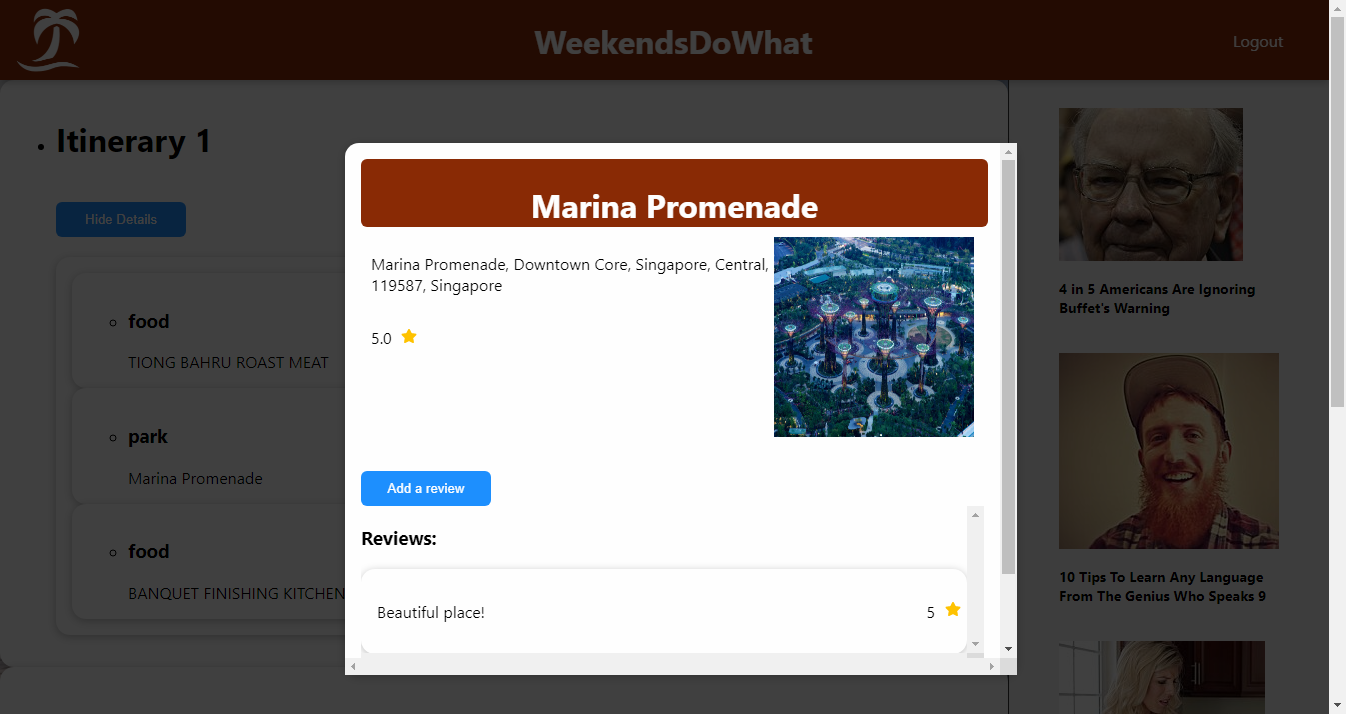
\includegraphics[width=1\textwidth]{figures/place-detail.png}
        	\caption{Viewing the details of a place}
        	\label{view_place_details}
        \end{figure}
        
        Premium users will be able to read the detailed reviews left by other premium users and can add their own reviews. Users can also use the feedback button to suggest ideas or suggest and edit on inaccurate or outdated information.
        
        \redfont{[User workflow diagram]}\todo{To be given by Pranav}
    
        \subsubsection{Data Source and Data Cleaning}
        
        For data integrity, consistency and reliability, we obtained our datasets from the trusted \url{data.gov.sg} and primarily selected two datasets on \href{https://data.gov.sg/dataset/eating-establishments}{eating establishments} and \href{https://data.gov.sg/dataset/parks}{parks} in Singapore for our application. Rather than having many datasets, we decided to start with these two and clean them well as we want to have reliable data and avoid a ‘garbage-in-garbage-out’ situation when we provide our solutions to our users.

        Providing high quality itinerary recommendations requires clean and high quality datasets. We carefully vetted the datasets chosen and cleaned the data in various ways, for example, removing data with missing values, selecting only the critical fields/columns and renaming of similar words for consistency.
        
        We also noticed that datasets from the government weren’t updated periodically and some of the latest versions were from two years ago. Consequently, we provide a feedback button for users to provide new information and report any out-of-date or inaccurate information in the data. We further enhanced the data points by integrating with additional Python libraries to provide an image to each location of our suggestion.


        \subsubsection{Frontend, Application and Database}
        
        Similar to a typical 3-tier application model, we built our frontend using ReactJS to provide a modern and responsive user experience and our backend application using Flask to provide APIs and implement the business logic. As our data naturally fits the relational data model, we used PostgreSQL as our database for data storage. We also carefully designed our SaaS application to be stateless to support multi-tenancy. We will cover the application deployment in detail in the section on AWS services deployed.

        To provide high quality itinerary recommendations, we rely on a few techniques and heuristics. We select places for users to visit and rank them first based on their distances from the user’s location, and adjust them by accounting for the overall ratings given by past visitors. Also, one common pattern we observe is that people like to have meals between different activities, therefore our recommendations also follow this pattern.


    \subsection{SaaS Design and Architecture}
    \autoref{deployment_architecture} illustrates our SaaS architecture design and we will describe how our application is designed and what AWS services are deployed in the sub-sections.
    
    \begin{figure}[H]
    	\centering
    	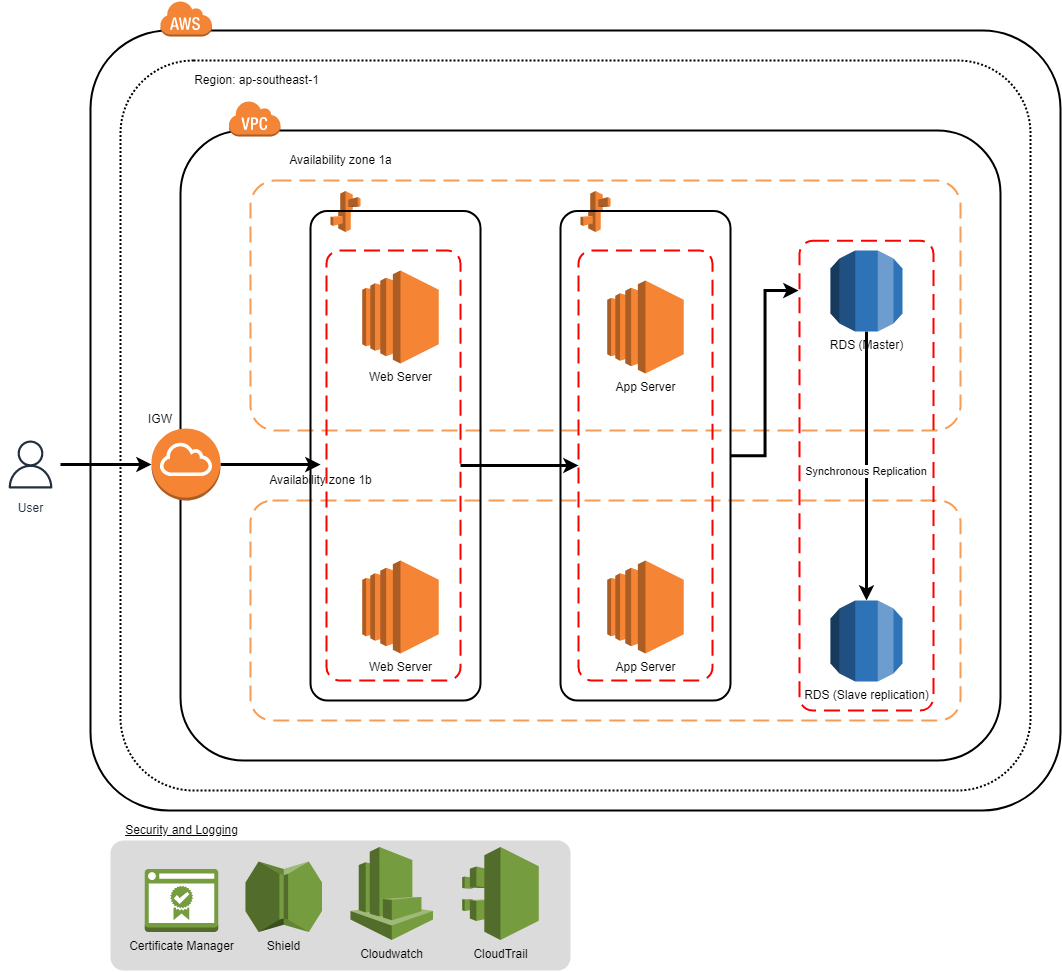
\includegraphics[width=1\textwidth]{figures/final.drawio.png}
    	\caption{SaaS Deployment Architecture}
    	\label{deployment_architecture}
    \end{figure}
    
        \label{section-aws-services-deployed}
        \subsubsection{AWS Services Deployed}
        
        For readability, we will bold the font of the AWS services we utilized for our SaaS application.

        For our SaaS application deployment, we use AWS services extensively from end-to-end. We set up our \textbf{Virtual Private Cloud (VPC)} within the ap-southeast-1 region, Singapore, as our targeted users are people exploring places in Singapore and attached an \textbf{Internet gateway (IGW)} to our VPC for public access.
        
        Within the VPC, we set up two \textbf{Elastic Beanstalk} to host our frontend and backend application. We also configured the \textbf{Auto scaling group} in our elastic beanstalks to spread across two \textbf{Availability Zones (AZ)}, illustrated with yellow dotted lines, zone 1a and 1b, with minimum instances count of 2 to ensure there is one EC2 instance in each AZ. The \textbf{S3 bucket}, \textbf{Load Balancer}, \textbf{Security Groups}, illustrated with red dotted lines, and \textbf{Cloudwatch} alarms are automatically set up when we launch the elastic beanstalk for our frontend and backend application. Additionally, we configured the security group of the backend application of the elastic beanstalk to only allow ingress traffic for HTTP (port 80) from the frontend’s security group. The S3 bucket is used to archive the application versions deployed on each elastic beanstalk.
        
        AWS provided a compatible range of services which enables our SaaS application to be more secure and most importantly, the basic services we used are free. We created a SSL certificate via the \textbf{AWS Certificate Manager} for our frontend elastic beanstalk so that all public traffic will use HTTPS protocol to communicate with our frontend elastic beanstalk. The SSL/TLS certificate provisioned through Certificate Manager is free. CloudTrail is automatically enabled and records every activity occurring in our elastic beanstalks. We can easily view, search, and download recent \textbf{CloudTrail} events along with other AWS service events in Event history. \textbf{AWS Shield Standard} is also available to provide protection and support high availability for our SaaS application. 
        
        For our PostgreSQL database, we deployed \textbf{Aurora PostgreSQL with multi-AZ} and database deletion protection enabled, having a writer replica in ap-southeast-1a zone and a  reader replica in ap-southeast-1b zone. Security group for our database is automatically created during the initial database creation and we configured additional ingress traffic for RDS (port 5432) from the backend application’s security group on our database’s security group. 
        
        \subsubsection{System Considerations}
        
        While there are advantages and disadvantages of using cloud over on-premise for our SaaS application, the advantages outweigh the disadvantages for our business case. We were able to save cost on on-premise equipment and additional employment of engineers to maintain the infrastructure. We can focus on the development and deliveries of our SaaS application, rather than spending time to set up and manage the infrastructure. Using cloud services also allows us to pay on-demand. We also do not have to worry and can rely on the cloud platform for our business continuity and disaster recovery strategy. We will dive into details for each system component and provide our design considerations for our SaaS application.
        
            \textbf{Systems}
            
            \textit{AWS Elastic beanstalk as our frontend and backend application deployments}
            
            We decided to use AWS Elastic beanstalk as our application stack as it automates the setup, configuration, and provisioning of other AWS services like EC2 instances, S3 bucket, security groups, Cloudwatch alarms and Elastic Load Balancing. This PaaS is free and we only need to pay for the AWS services we used for our SaaS application. Elastic beanstalk also enables easy deployment of new application versions through AWS CLI. As most of us are new to cloud computing, this PaaS allows us to deploy and manage our application within minutes in the AWS cloud.
            
            \textit{Aurora PostgreSQL as our database}
            
            We decided to use Aurora PostgreSQL-Compatible Edition over Amazon RDS PostgreSQL due to a number of factors. Aurora's unique architecture gives us more durability, scale and resilience despite being more costly than AWS RDS PostgreSQL.

            For performance, Aurora PostgreSQL performs better than Amazon RDS PostgreSQL in throughput as it uses shared storage for the writer and readers replicas and allows scaling storage across the two AZs we used in the region. Amazon Aurora gives two times the throughput provided by RDS PostgreSQL or five times the throughput provided by standard MySQL running on similar hardware. Aurora PostgreSQL allows provisioning up to 15 replicas, and the replication is done in milliseconds. On the other hand, RDS PostgreSQL only allows five replicas, and the process of replication is slower compared to Amazon Aurora.
            
            For disaster recovery,  failover is done automatically to prevent data loss.
            
            \textit{Availability}
            
            Elastic Beanstalk includes an Auto Scaling group that manages the Amazon EC2 instances in our environment. In a load-balanced environment, we configured the group with a range of instances to run, and Auto Scaling adds or removes instances as needed, based on load. The Auto Scaling group used two Amazon CloudWatch alarms to trigger scaling operations. We are able to configure triggers that are appropriate for our application, instance type, and service requirements and scale based on several statistics including latency, disk I/O, CPU utilization, and request count. For our SaaS, the most computational expensive part is itinerary generation. Thus, in order to achieve a server response time less than 100ms, we would add an additional EC2 instance if CPU utilization for backend exceeds 80\%. Additionally, the Auto Scaling monitors the health of each Amazon EC2 instance that it launches. If any instance terminates unexpectedly, Auto Scaling detects the termination and launches a replacement instance.

            \textit{Network}
            
            We deployed our SaaS application via elastic beanstalks on multi AZ to ensure availability and configure our database with multi-AZ replication on a separate AZ for data recovery.
            
            \textit{Security}
            
            We secure our application with the use of multiple AWS components as described below:
            \begin{itemize}
                \item Security groups and policies created with permissions for our frontend, backend server and database to securely talk to each other. All the servers are configured so they can only talk to and have permissions for what they need.
                \item Basic monitoring of our servers through Cloudwatch.
                \item Logging Amazon Route 53 API calls with AWS CloudTrail.
                \item AWS Shield Standard to protect against common and most frequently occurring infrastructure (layer 3 and 4) attacks like SYN/UDP floods, reflection attacks, and others to support high availability.
            \end{itemize}
            
            \textit{Data and Recovery}
            
            Our Aurora PostgreSQL is deployed with multi-AZ data replication and failover is done automatically to prevent data loss. This allows us to achieve a shorter Recovery time objective (RTO) and faster Recovery point objective (RPO) for Business continuity and Disaster Recovery (BC/DR).

        \subsubsection{Limitations}
        
        Using elastic beanstalk also comes with its limitations. Our deployments would take 5 minutes at least and sometimes stretch to 15 minutes. We noticed with more servers, deployments could take even longer. With every new version deployment, Elastic Beanstalk archives the old application version in an S3 bucket. We learned to occasionally delete old application versions to prevent deployment failures.

        Our workload can be considerably small to medium and for this case, using AWS Aurora PostgreSQL is more costly than AWS RDS PostgreSQL. It is only cost effective if we have high workloads, and with that, using Aurora is cheaper and faster than running the equivalent RDS database.
        
        We hope we can provide a better SaaS in future if more time permits by enhancing our deployment process with Docker containers to add more versatility.

\section{Economic Factors}

Since AWS has its own servers and database in Singapore, so even if users ask to have their data stored locally, we could still utilize the AWS RDS service. The only advantage for on-premise IT resources is that we have full control of the hardware and could perform security updates as soon as possible. We have noticed that AWS elastic beanstalk doesn’t support many of the latest packages and language updates, which could cause security vulnerabilities like the recent Log4j. However, as illustrated in the Business Model section, the cost of hiring IT staff in Singapore would exceed the cost of AWS. Moreover, we expect to have rapid user growth in the first few months, so using cloud service could provide the elasticity to expand our business. With current global chip shortages and delay in logistics, newly purchased on-premise servers might not arrive in time. Thus, despite the few disadvantages of AWS, deploying our SaaS on cloud service is the more feasible way.

Since we don’t think there would be a fixed minimum number of user accesses throughout the day, we would not opt for reserved instances on AWS. With our configuration on elastic beanstalk, we will only have 2 instances for frontend and backend respectively during off-peak hours, which will cost us a total of \$1.0144 per hour. Compared with on-demand pricing, cost reduction of 1-year reserved small instances is negligible. For ease of development and higher reliability, all of our instances are based on x86 processors currently. As more software improves their performance and compatibility on ARM based processors, we could immediately switch to cheaper and higher performance ARM instances on AWS if we opt for on-demand pricing for all of our instances.

We also considered using AWS Lambda for our backend, because it is serverless and more agile than Elastic Beanstalk. However, we discovered that AWS Lambda would take more than 2 seconds to respond if the trigger function has been inactive for a long time.In order to reduce the latency of AWS Lambda to less than 100 ms, we have to constantly ping the functions even if no users are using the service. This significantly increased our cost for using AWS Lambda to \$850 per month, which is \$166.14 more than using Elastic Beanstalk for backend. 

\section{Conclusion}

AWS cloud has been a great enabler in allowing our team to deliver our business model in a relatively short amount of time by focusing on the features, rather than managing the infrastructure or platforms. AWS services come with a variety of AI/ML and security tools which we have benefited from such as the AWS CloudTrail, AWS Cloudwatch and AWS shield to secure our application from malicious actors. AWS cloud also helped us to reduce cost effectively as we are required to pay as per demand and we can choose which AWS services appropriately for our SaaS after a thorough cost analysis with their AWS cost estimation. 

We hope that our SaaS will be able to provide more recommendations for locals to explore local parks and eateries and be the most attractive platform used by people as the Covid-19 measures ease in Singapore. 

We also would like to give thanks and appreciation to our professor Teo Yong Meng, Dumitrel Loghin and the entire teaching staff for providing useful feedback during our consultations.

\end{document}
